%%%%%%%%%%%%%%%%%%%%%%%%%%%%%%%%%%%%%%%%%%%%%%%%%%%%%%%%%%%%%%%%%%%%%%
%%  Copyright by Wenliang Du.                                       %%
%%  This work is licensed under the Creative Commons                %%
%%  Attribution-NonCommercial-ShareAlike 4.0 International License. %%
%%  To view a copy of this license, visit                           %%
%%  http://creativecommons.org/licenses/by-nc-sa/4.0/.              %%
%%%%%%%%%%%%%%%%%%%%%%%%%%%%%%%%%%%%%%%%%%%%%%%%%%%%%%%%%%%%%%%%%%%%%%

\newcommand{\commonfolder}{../../common-files}
\input{\commonfolder/header}
\input{\commonfolder/copyright}

\lhead{\bfseries SEED Labs -- Smurf and Fraggle Attack Lab}

\newcommand{\smurflab}{\texttt{Smurf/Fraggle}\xspace}
\newcommand{\attacker}{\texttt{AS-150}\xspace}
\newcommand{\victim}{\texttt{AS-151}\xspace}
\newcommand{\amplifier}{\texttt{AS-152}\xspace}
\newcommand{\fraggleport}{\texttt{7000}\xspace}

\begin{document}

\begin{center}
{\LARGE Smurf and Fraggle Attack Lab}
\end{center}

\seedlabcopyright{2026}


% *******************************************
% SECTION
% *******************************************
\section{Overview}

Smurf and Fraggle attacks are reflection and amplification attacks. In these
attacks, the attacker sends packets to a broadcast address, but spoofs the
source address to be the victim's address. The machines on the broadcast
network reply to the victim, so one spoofed packet from the attacker can trigger
many packets toward the victim. The Smurf attack uses ICMP echo request packets;
the Fraggle attack follows the same pattern using UDP packets.

The objective of this lab is to help students understand the common pattern
behind these attacks: IP spoofing, directed broadcast, reflection, and
amplification. Students will write their own packet-sending programs, observe
the reflected traffic, measure the amplification effect, and test several
defense mechanisms. This lab covers the following topics:

\begin{itemize}[noitemsep]
\item IP spoofing and packet reflection
\item Directed broadcast and broadcast forwarding
\item ICMP echo request and echo reply
\item UDP-based reflection using a simple responder
\item Packet observation using \texttt{tcpdump} and \texttt{netcat}
\item Defense mechanisms against reflection and amplification
\end{itemize}


\paragraph{Readings and Videos.}
Detailed coverage of the IP protocol, ICMP, packet spoofing, and denial-of-service
attacks can be found in the following:

\begin{itemize}
\item Chapter 3 of the SEED Book, \seedisbook
\item Section 4 of the SEED Lecture, \seedisvideo
\end{itemize}


\paragraph{Lab environment.}
\seedenvironmentB
\nodependency


\paragraph{Ethics and safety.}
The attacks in this lab must only be conducted inside the provided SEED
emulator. Students should not send spoofed packets or broadcast packets to
networks outside the lab environment.


% *******************************************
% SECTION
% *******************************************
\section{The Lab Setup and the SEED Internet Emulator}

This lab is conducted inside the SEED Internet Emulator. We use a small
emulated Internet with five stub autonomous systems (ASes). The lab uses three
of them:

\begin{itemize}[noitemsep]
\item \attacker: the attacker host. Students write and run their attack programs
      from this host.
\item \victim: the victim host. Students observe reflected ICMP and UDP traffic
      on this host.
\item \amplifier: the amplifier LAN. Directed broadcast is enabled on the router
      of this AS. Multiple hosts on this LAN will reply to broadcast traffic.
\end{itemize}

The important addresses used in the lab are listed below. The exact container
names can be found using the \texttt{dockps} command after the emulator starts.

\begin{center}
\begin{tabular}{|l|l|l|}
\hline
\textbf{Role} & \textbf{Node} & \textbf{Address} \\
\hline
Attacker & \texttt{as150h-host\_0} & \texttt{10.150.0.71} \\
Victim & \texttt{as151h-host\_0} & \texttt{10.151.0.71} \\
Amplifier router & \texttt{as152r-router0} & \texttt{10.152.0.254} \\
Amplifier broadcast address & \texttt{AS-152 net0} & \texttt{10.152.0.255} \\
Amplifier hosts & \texttt{as152h-host\_*} & \texttt{10.152.0.71}, \texttt{10.152.0.72}, \ldots \\
\hline
\end{tabular}
\end{center}


\subsection{Starting the Emulator}

\input{\commonfolder/emulator/setup}

For this lab, the container files are generated in the \texttt{Labsetup/output}
folder. Go to this folder and start the emulator:

\begin{lstlisting}
$ cd Labsetup/output
$ docker-compose build
$ docker-compose up
\end{lstlisting}

In another terminal, use the following commands to find and enter the relevant
containers:

\begin{lstlisting}
$ dockps | grep Attacker      # Attacker
$ dockps | grep as151      # Victim
$ dockps | grep as152      # Amplifier router and hosts

$ docksh <container-id>
\end{lstlisting}

The attacker host already has \texttt{python3}, \texttt{Scapy}, and
\texttt{tcpdump}. The victim host has \texttt{tcpdump} and
\texttt{netcat-openbsd}. Each amplifier host runs a small UDP responder on port
\fraggleport for the Fraggle experiment.


\subsection{Changing the Emulator Parameters}

Instructors can customize the lab by regenerating the container files from
\texttt{Labsetup/emulator.py}. The script has a few command
line options. Changing \texttt{--amplifier-hosts} is a convenient way to change the
amplification factor. 

\begin{lstlisting}
$ python3 emulator.py --platform amd
$ python3 emulator.py --platform arm
$ python3 emulator.py --hosts-per-as 1
$ python3 emulator.py --amplifier-hosts 20
$ python3 emulator.py --fraggle-port 7000
\end{lstlisting}



% *******************************************
% SECTION
% *******************************************
\section{Theory}
\label{sec:theory}

\subsection{Directed Broadcast}

In an IPv4 network, the last address of a subnet is normally the broadcast
address. For example, for the network \texttt{10.152.0.0/24}, the broadcast
address is \texttt{10.152.0.255}. A packet sent to this address is delivered to
all hosts on that LAN.

A directed broadcast packet is a packet sent from outside a network to that
network's broadcast address. If the router forwards the packet into the target
LAN as a broadcast frame, many hosts can receive the same packet. Because this
behavior can be abused for amplification attacks, modern networks usually block
directed broadcast by default.


\subsection{Reflection and Amplification}

In a reflection attack, the attacker does not send the final traffic directly to
the victim. Instead, the attacker sends requests to reflectors and spoofs the
source IP address to be the victim's address. The reflectors send their replies
to the victim.

In an amplification attack, a small amount of attacker traffic causes a larger
amount of victim traffic. With directed broadcast, one packet can be delivered
to many hosts. If every host replies to the spoofed source address, the victim
receives many replies. If there are \(N\) responding hosts, one request can
produce approximately \(N\) replies.




\subsection{The Smurf Attack}

The Smurf attack uses ICMP. The attacker sends an ICMP echo request to the
directed broadcast address and spoofs the source IP address to be the victim's
address. Each amplifier host receives the echo request and sends an ICMP echo
reply to the victim. Figure~\ref{fig:smurf-attack} illustrates the attack.

\begin{figure}[htb]
\begin{center}
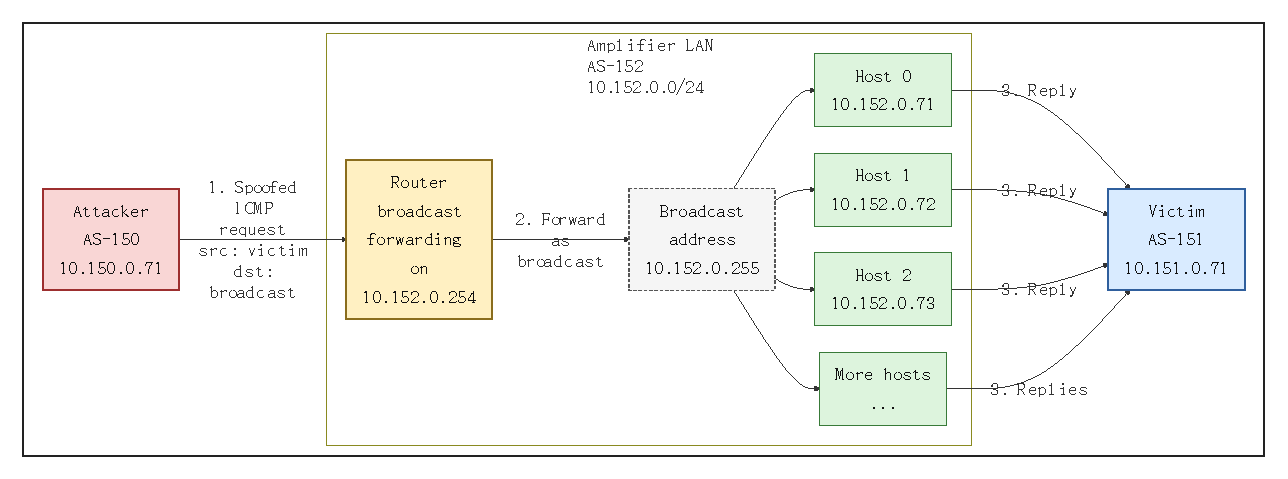
\includegraphics[width=0.95\textwidth]{Figs/smurf_attack.pdf}
\end{center}
\vspace{-0.2in}
\caption{Smurf attack}
\label{fig:smurf-attack}
\end{figure}
 

The attacker does not need to receive the replies. The main observable effect is
on the victim, which receives a burst of ICMP echo replies from many amplifier
hosts.


\subsection{The Fraggle Attack}

The Fraggle attack follows the same reflection pattern, but uses UDP instead of
ICMP. In the emulator, amplifier hosts run a simple UDP responder on port
\fraggleport. When they receive a UDP packet on this port, they send a response
to the source IP address and source UDP port in the request.

To make the victim receive the reflected UDP replies, the attacker must spoof
the packet's source IP address as the victim's address. If the victim runs
\texttt{nc -ul 7000}, the attacker should also choose UDP source port
\fraggleport, so the replies are delivered to the victim's listening port.


\subsection{Defenses}

There are several places to stop this attack pattern:

\begin{itemize}[noitemsep]
\item Routers can disable directed broadcast forwarding.
\item Hosts can ignore ICMP echo requests sent to broadcast addresses.
\item Networks can apply ingress/egress filtering to block packets with spoofed
      source addresses.
\item Services can avoid sending large unauthenticated replies to small UDP
      requests.
\end{itemize}

In this lab, students will test router-side and host-side defenses inside the
emulator.


% *******************************************
% SECTION
% *******************************************
\section{Lab Tasks}


% -------------------------------------------
% SUBSECTION
% -------------------------------------------
\subsection{Task 1: Inspecting the Lab Environment}

The objective of this task is to become familiar with the emulator topology and
connect it to the theory of directed broadcast. 

Start the emulator and find the attacker, victim, amplifier router, and several
amplifier hosts. Use the following commands to find and enter the relevant containers:

\begin{lstlisting}
$ dockps | grep -i attacker   # Attacker
$ dockps | grep -i victim     # Victim
$ dockps | grep -i as152      # Amplifier router and hosts

$ docksh <container-id>       # Enter the container
\end{lstlisting}

On the victim, start a packet capture for ICMP traffic:

\begin{lstlisting}
# tcpdump -n -i any icmp
\end{lstlisting}

On the attacker, send a normal ping to the victim and to one amplifier host.
Then try to ping the AS-152 broadcast address:

\begin{lstlisting}
# ping -c 3 10.151.0.71
# ping -c 3 10.152.0.71
# ping -c 3 10.152.0.255
\end{lstlisting}

Please report your observations. How many replies do you see when the
broadcast address is used? Which theory from Section~\ref{sec:theory}
explains this behavior?


% -------------------------------------------
% SUBSECTION
% -------------------------------------------
\subsection{Task 2: Writing a Smurf Attack Program}

The objective of this task is to implement the Smurf attack by constructing a
spoofed ICMP packet. Students must write their own program on the attacker host
using Scapy.

Your program should send an ICMP echo request to the AS-152 directed broadcast
address. The source IP address of the packet should be the victim's IP address.
The following skeleton shows the structure of the program. Important values are
intentionally left blank.

\begin{lstlisting}[language=python]
#!/usr/bin/env python3
from scapy.all import *

victim_ip = "..."
broadcast_ip = "..."

ip = IP(src=..., dst=...)
icmp = ICMP(type=...)
payload = b"..."

packet = ip/icmp/payload
send(packet, verbose=0)
\end{lstlisting}

You can edit the program on the host machine using an editor, such as 
vi, gedit, or vscode, and then using \texttt{"docker copy"} to 
copy the program from the host to the container. 


Run \texttt{tcpdump} on the victim before launching the attack:

\begin{lstlisting}
# tcpdump -n -i any icmp
\end{lstlisting}

Then run your attack program from the attacker. Please demonstrate that the
victim receives ICMP echo replies from multiple amplifier hosts. In your lab
report, explain why the replies go to the victim instead of the attacker.



% -------------------------------------------
% SUBSECTION
% -------------------------------------------
\subsection{Task 3: Measuring the Smurf Amplification Effect}

The objective of this task is to connect the attack result back to the theory of
amplification.

Modify your Smurf program so it sends a chosen number of spoofed ICMP echo
requests, with a short delay between packets. On the victim, use
\texttt{tcpdump} to count the number of ICMP echo replies received.

\begin{lstlisting}
# tcpdump -n -i any 'icmp and src net 10.152.0.0/24'
\end{lstlisting}

Run the experiment with different numbers of amplifier hosts. If your instructor
provides several versions of the emulator, compare the results. If not, record
the number of amplifier hosts in the current emulator and estimate the expected
number of replies.

Please include the following in your report:

\begin{itemize}[noitemsep]
\item The number of spoofed requests sent by the attacker.
\item The number of amplifier hosts that replied.
\item The number of replies observed by the victim.
\item Whether the observed result matches the amplification theory.
\end{itemize}



% -------------------------------------------
% SUBSECTION
% -------------------------------------------
\subsection{Task 4: Writing a Fraggle Attack Program}

The objective of this task is to show that the same reflection pattern can be
applied to UDP traffic.

On the victim, start a UDP listener using \texttt{netcat}. It will print the
payloads of UDP packets delivered to port \fraggleport.

\begin{lstlisting}
# nc -ul 7000
\end{lstlisting}

On the attacker, write a Scapy program that sends a UDP packet to the AS-152
broadcast address and port \fraggleport. The packet's source IP address should
be the victim's IP address. To make the victim's \texttt{netcat} listener
receive the replies, use source UDP port \fraggleport.

\begin{lstlisting}[language=python]
#!/usr/bin/env python3
from scapy.all import *

victim_ip = "..."
broadcast_ip = "..."
port = ...

ip = IP(src=..., dst=...)
udp = UDP(sport=port, dport=port)
payload = b"..."

packet = ip/udp/payload
send(packet, verbose=0)
\end{lstlisting}

Please demonstrate that the victim receives UDP payloads from the amplifier
hosts. Explain why the UDP source port matters in this task.



% -------------------------------------------
% SUBSECTION
% -------------------------------------------
\subsection{Task 5: Defense 1 -- Disabling Directed Broadcast}

The objective of this task is to test the most direct defense against the attack
pattern described in Section 3.

Get a shell on the AS-152 router and disable broadcast forwarding. Different
Linux kernels expose this control in slightly different ways, so students should
try the following commands and then verify the values under
\texttt{/proc/sys/net/ipv4/conf/}.

\begin{lstlisting}
# sysctl -w net.ipv4.conf.all.bc_forwarding=0
# sysctl -w net.ipv4.conf.default.bc_forwarding=0
# for f in /proc/sys/net/ipv4/conf/*/bc_forwarding; do echo 0 > $f; done
\end{lstlisting}

Run your Smurf and Fraggle attack programs again. Please report whether the
victim still receives reflected traffic. Explain why this defense works or does
not work, using the directed broadcast theory.


% -------------------------------------------
% SUBSECTION
% -------------------------------------------
\subsection{Task 6: Defense 2 -- Disabling ICMP Broadcast Replies}

The objective of this task is to test a host-side defense and compare it with
the router-side defense.


On each amplifier host, configure Linux to ignore ICMP echo requests sent to a
broadcast address. Since the emulator may contain many amplifier hosts, we
provide a script in the \texttt{Labsetup} folder to apply the configuration to
all AS-152 host containers:

\begin{lstlisting}
$ cd Labsetup
$ ./bcast-reply.sh off     # Turn off the broadcast reply 
$ ./bcast-reply.sh on      # Turn on the broadcast reply 
$ ./bcast-reply.sh status  # Show the status
\end{lstlisting}

The script runs the following command inside each amplifier host container:

\begin{lstlisting}
# sysctl -w net.ipv4.icmp_echo_ignore_broadcasts=1
\end{lstlisting}

Run the Smurf attack again and observe the victim. Then run the Fraggle attack
again. Please answer the following questions:

\begin{itemize}[noitemsep]
\item Does this defense stop the Smurf attack?
\item Does this defense stop the Fraggle attack?
\item Why is the result different for ICMP and UDP?
\item Which defense is more general for this lab: disabling directed broadcast
      or disabling ICMP broadcast replies?
\end{itemize}


% *******************************************
% SECTION
% *******************************************
\section{Guidelines}

\subsection{Running Scapy Programs}

Raw packet spoofing requires root privilege. Inside the SEED containers, the
shell normally runs as root, so students can directly execute their Python
programs:

\begin{lstlisting}
# python3 smurf.py
# python3 fraggle.py
\end{lstlisting}

If Scapy complains about missing permissions, make sure the program is executed
inside the attacker container and not on the host machine.


\subsection{Useful Tcpdump Filters}

The following filters are useful in this lab:

\begin{lstlisting}
# tcpdump -n -i any icmp
# tcpdump -n -i any 'icmp and src net 10.152.0.0/24'
# tcpdump -n -i any udp port 7000
# tcpdump -n -i any host 10.151.0.71
\end{lstlisting}

Students should use \texttt{-n} so \texttt{tcpdump} prints IP addresses instead
of trying to resolve names.


\subsection{Checking the UDP Responder on Amplifier Hosts}

The Fraggle part of this lab uses a small UDP responder running on amplifier
hosts. To check whether it is running, use the following commands on an
amplifier host:

\begin{lstlisting}
# ps aux | grep fraggle
# tail /var/log/fraggle-amplifier.log
\end{lstlisting}

Students do not need to modify this responder. The attack program should be
written on the attacker host.


\subsection{Common Problems}

\noindent\textbf{No reflected packets are observed.}
Check the destination and source addresses in the attack packet. The destination
should be the broadcast address \texttt{10.152.0.255}; the spoofed source
address should be the victim address \texttt{10.151.0.71}.

\paragraph{The victim's \texttt{netcat} does not show UDP payloads.}
Make sure \texttt{nc -ul 7000} is running before launching the Fraggle attack.
Also check whether your UDP packet uses source port \fraggleport; otherwise, the
amplifier replies may be sent to a different port on the victim.

\paragraph{The defense task seems to have no effect.}
Make sure the defense command is run on the correct node. Directed broadcast
forwarding should be disabled on the AS-152 router. ICMP broadcast replies
should be disabled on the amplifier hosts.


% *******************************************
% SECTION
% *******************************************
\section{Submission}

\seedsubmission

In addition, please include the following:

\begin{itemize}[noitemsep]
\item The source code of your Smurf and Fraggle attack programs, with
      explanations of the important packet fields.
\item Screenshots or terminal logs showing reflected ICMP replies on the victim.
\item Screenshots or terminal logs showing reflected UDP payloads on the victim.
\item Your amplification measurements and explanation.
\item Your defense experiments and explanation of why each defense works or
      fails.
\end{itemize}

\end{document}
